During the development phase, we wanted to ensure that our steps worked as expected and delivered the right functionality. Two main approaches were taken during development. One was the use of Gazebo simulation to verify that specific implementations met our expectations. However, we were aware that the simulation does not necessarily have to match the behavior of the actual platform.\\
\newline
For the car platform, we initially used pre-recorded rosbags from the F1TENTH system. Additionally, we managed to record multiple rosbags because ROS bags are large in size, and recording, for example, one with LiDAR but without the camera topics allowed for smoother testing of LiDAR-specific topics. This was one of the most efficient ways to test and analyze the vehicle’s response to real-world data.\\
\newline
In addition to simulation-based validation, a range of unit tests were implemented for multiple nodes during the developmental process. The purpose of these unit tests was to ensure the correctness of the functions within each node. These unit tests were designed to validate key components of the system, such as perception, control, and localization, by checking their outputs against expected values. The automation of these tests enabled the detection and rectification of issues, thereby we could ensure the reliability of the software.\\
\newline
Still, live testing was necessary in order to guarantee that the car's behavior in simulation translates into the real world. These tests took place in the AVAI lab space mostly during the weekly sprint meetings in the lecture period and also on an irregular basis in the lecture free period. During those tests the functionality of the current state of the stack was tested and reviewed. For this, one had to establish an SSH connection to the car. This connection enables the car to access our GitHub repository for synchronization and branch checkout, and the tester to start nodes or launch files on the car. \\
\newline
Most of these tests were documented in a short result protocol that was shared amongst the development team. For extensive debugging some protocols included the test setup and tasks as can be seen in Figure \ref{fig:protocol}.

\begin{figure}[htp]
	\vskip 0.2in
	\begin{center}
		\centerline{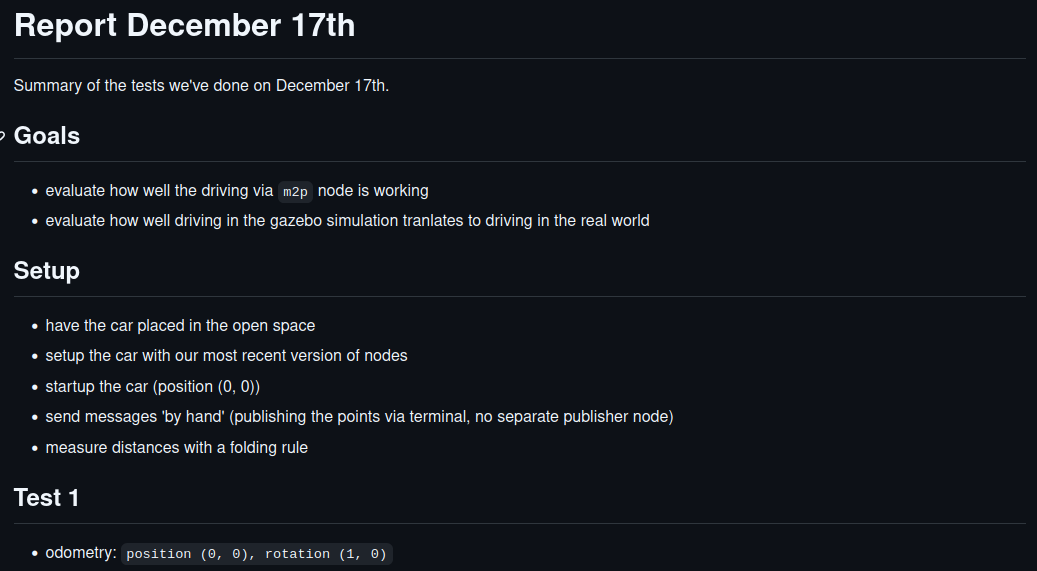
\includegraphics[width=\columnwidth]{protocol.png}}
		\caption{Screenshot of a test report.}
		\label{fig:protocol}
	\end{center}
	\vskip -0.2in
\end{figure}
